\section{Auswertung}
\label{sec:Auswertung}

\begin{figure}
  \centering
  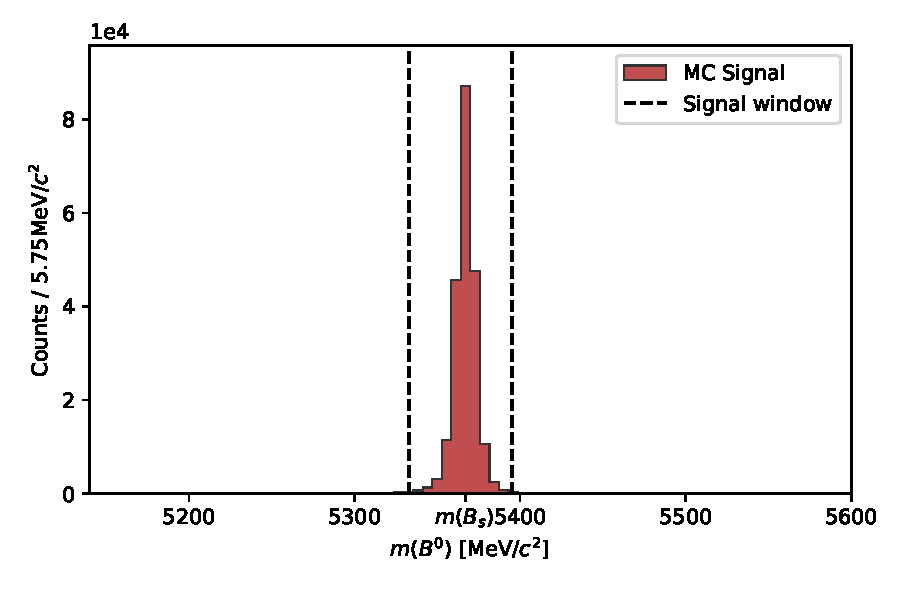
\includegraphics[width = .8\textwidth]{"content/plots/mass_signal.pdf"}
  \caption{Invariant mass distribution of the $B^0_s$ candidates for the signal channel simulation data.}
  \label{fig:mass_signal}
\end{figure}

\begin{figure}
  \centering
  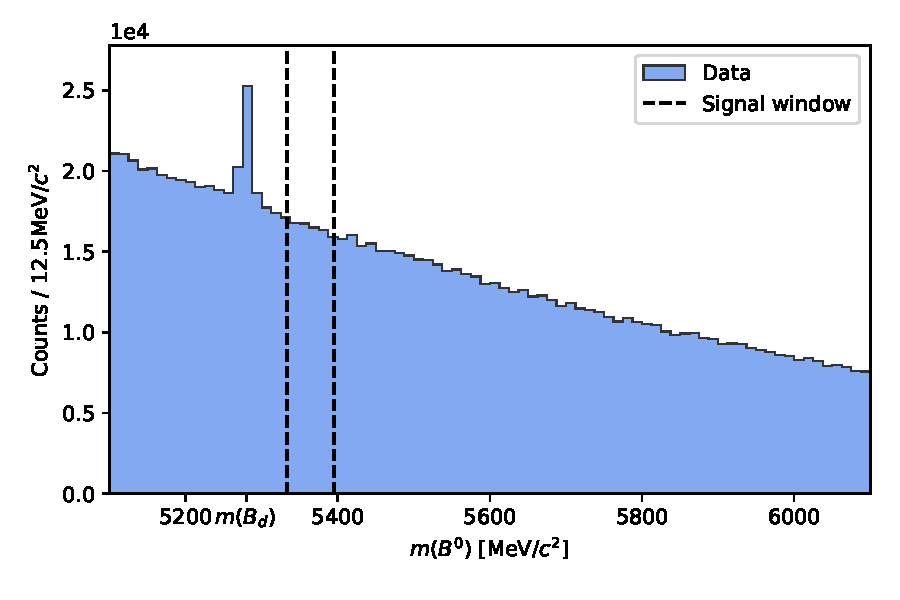
\includegraphics[width = .8\textwidth]{"content/plots/mass_data.pdf"}
  \caption{Invariant mass distribution of the $B^0$ candidates for the recorded LHCb data.}
  \label{fig:mass_data}
\end{figure}

\begin{figure}
  \centering
  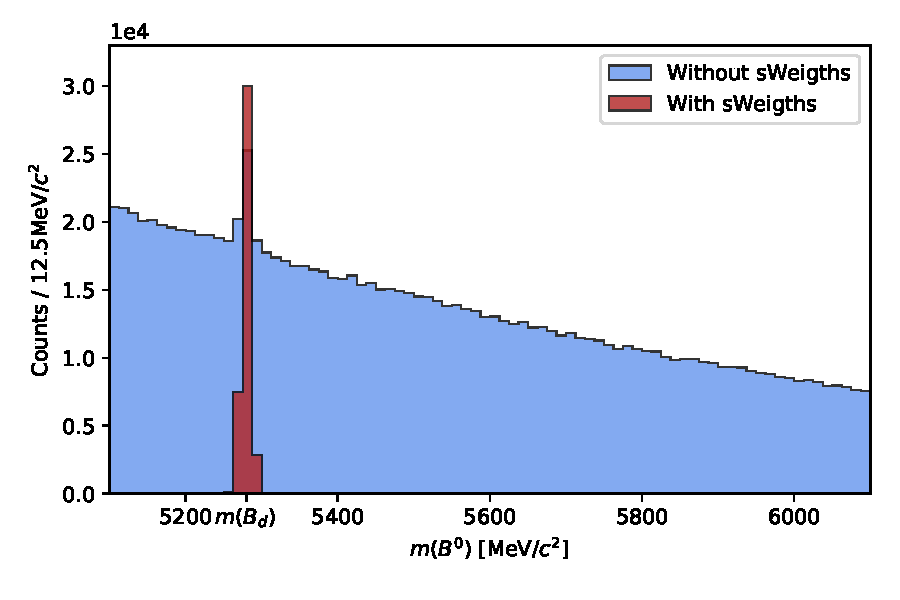
\includegraphics[width = .8\textwidth]{"content/plots/mass_reweighted.pdf"}
  \caption{Invariant mass distribution of the $B^0$ candidates for the recorded LHCb data and sWeights reweighted data.}
  \label{fig:mass_reweighted}
\end{figure}

\subsection{Feature selection}

\begin{figure}
  \centering
  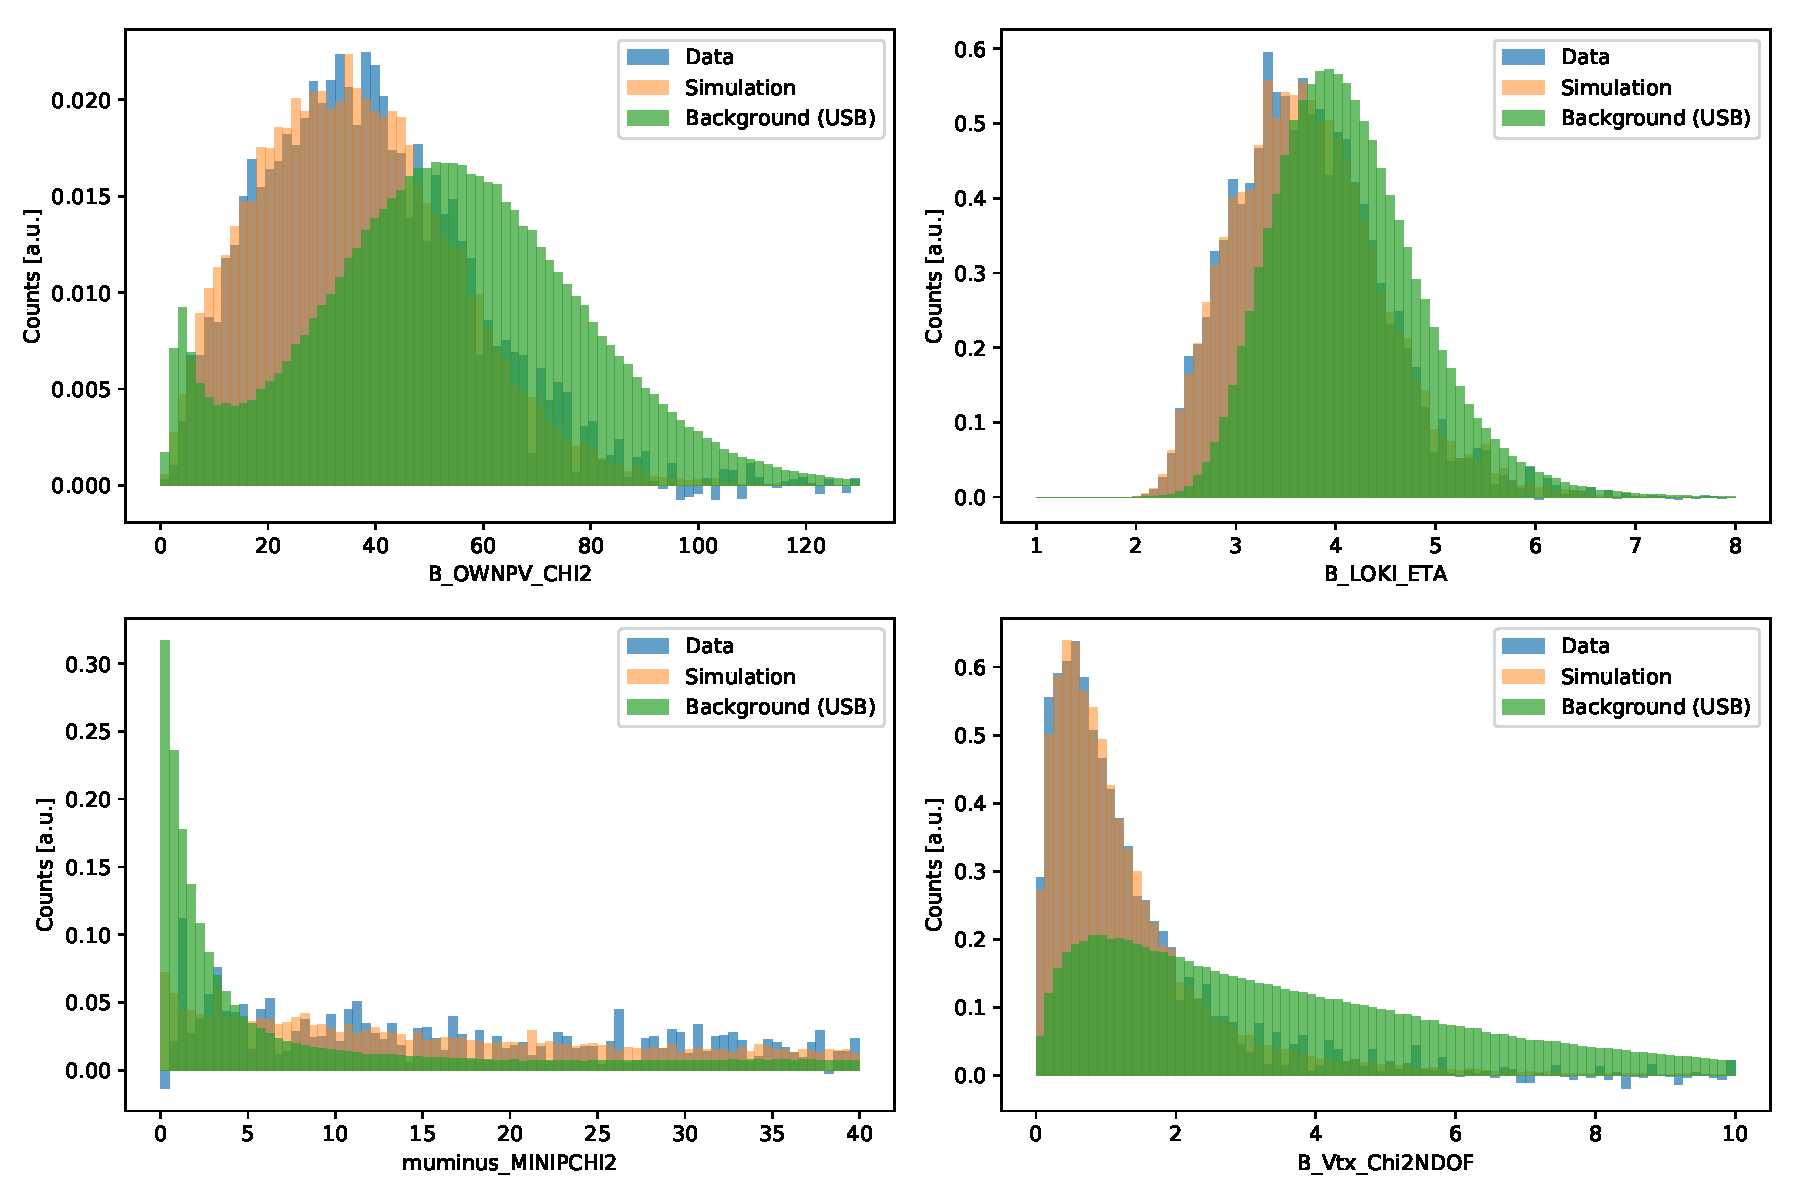
\includegraphics[width = .9\textwidth]{"content/plots/4variables.pdf"}
  \caption{Distributions of four selected variables used in the MVA for simulation, reweighted data and background.}
  \label{fig:4variables}
\end{figure}

\begin{figure}
  \centering
  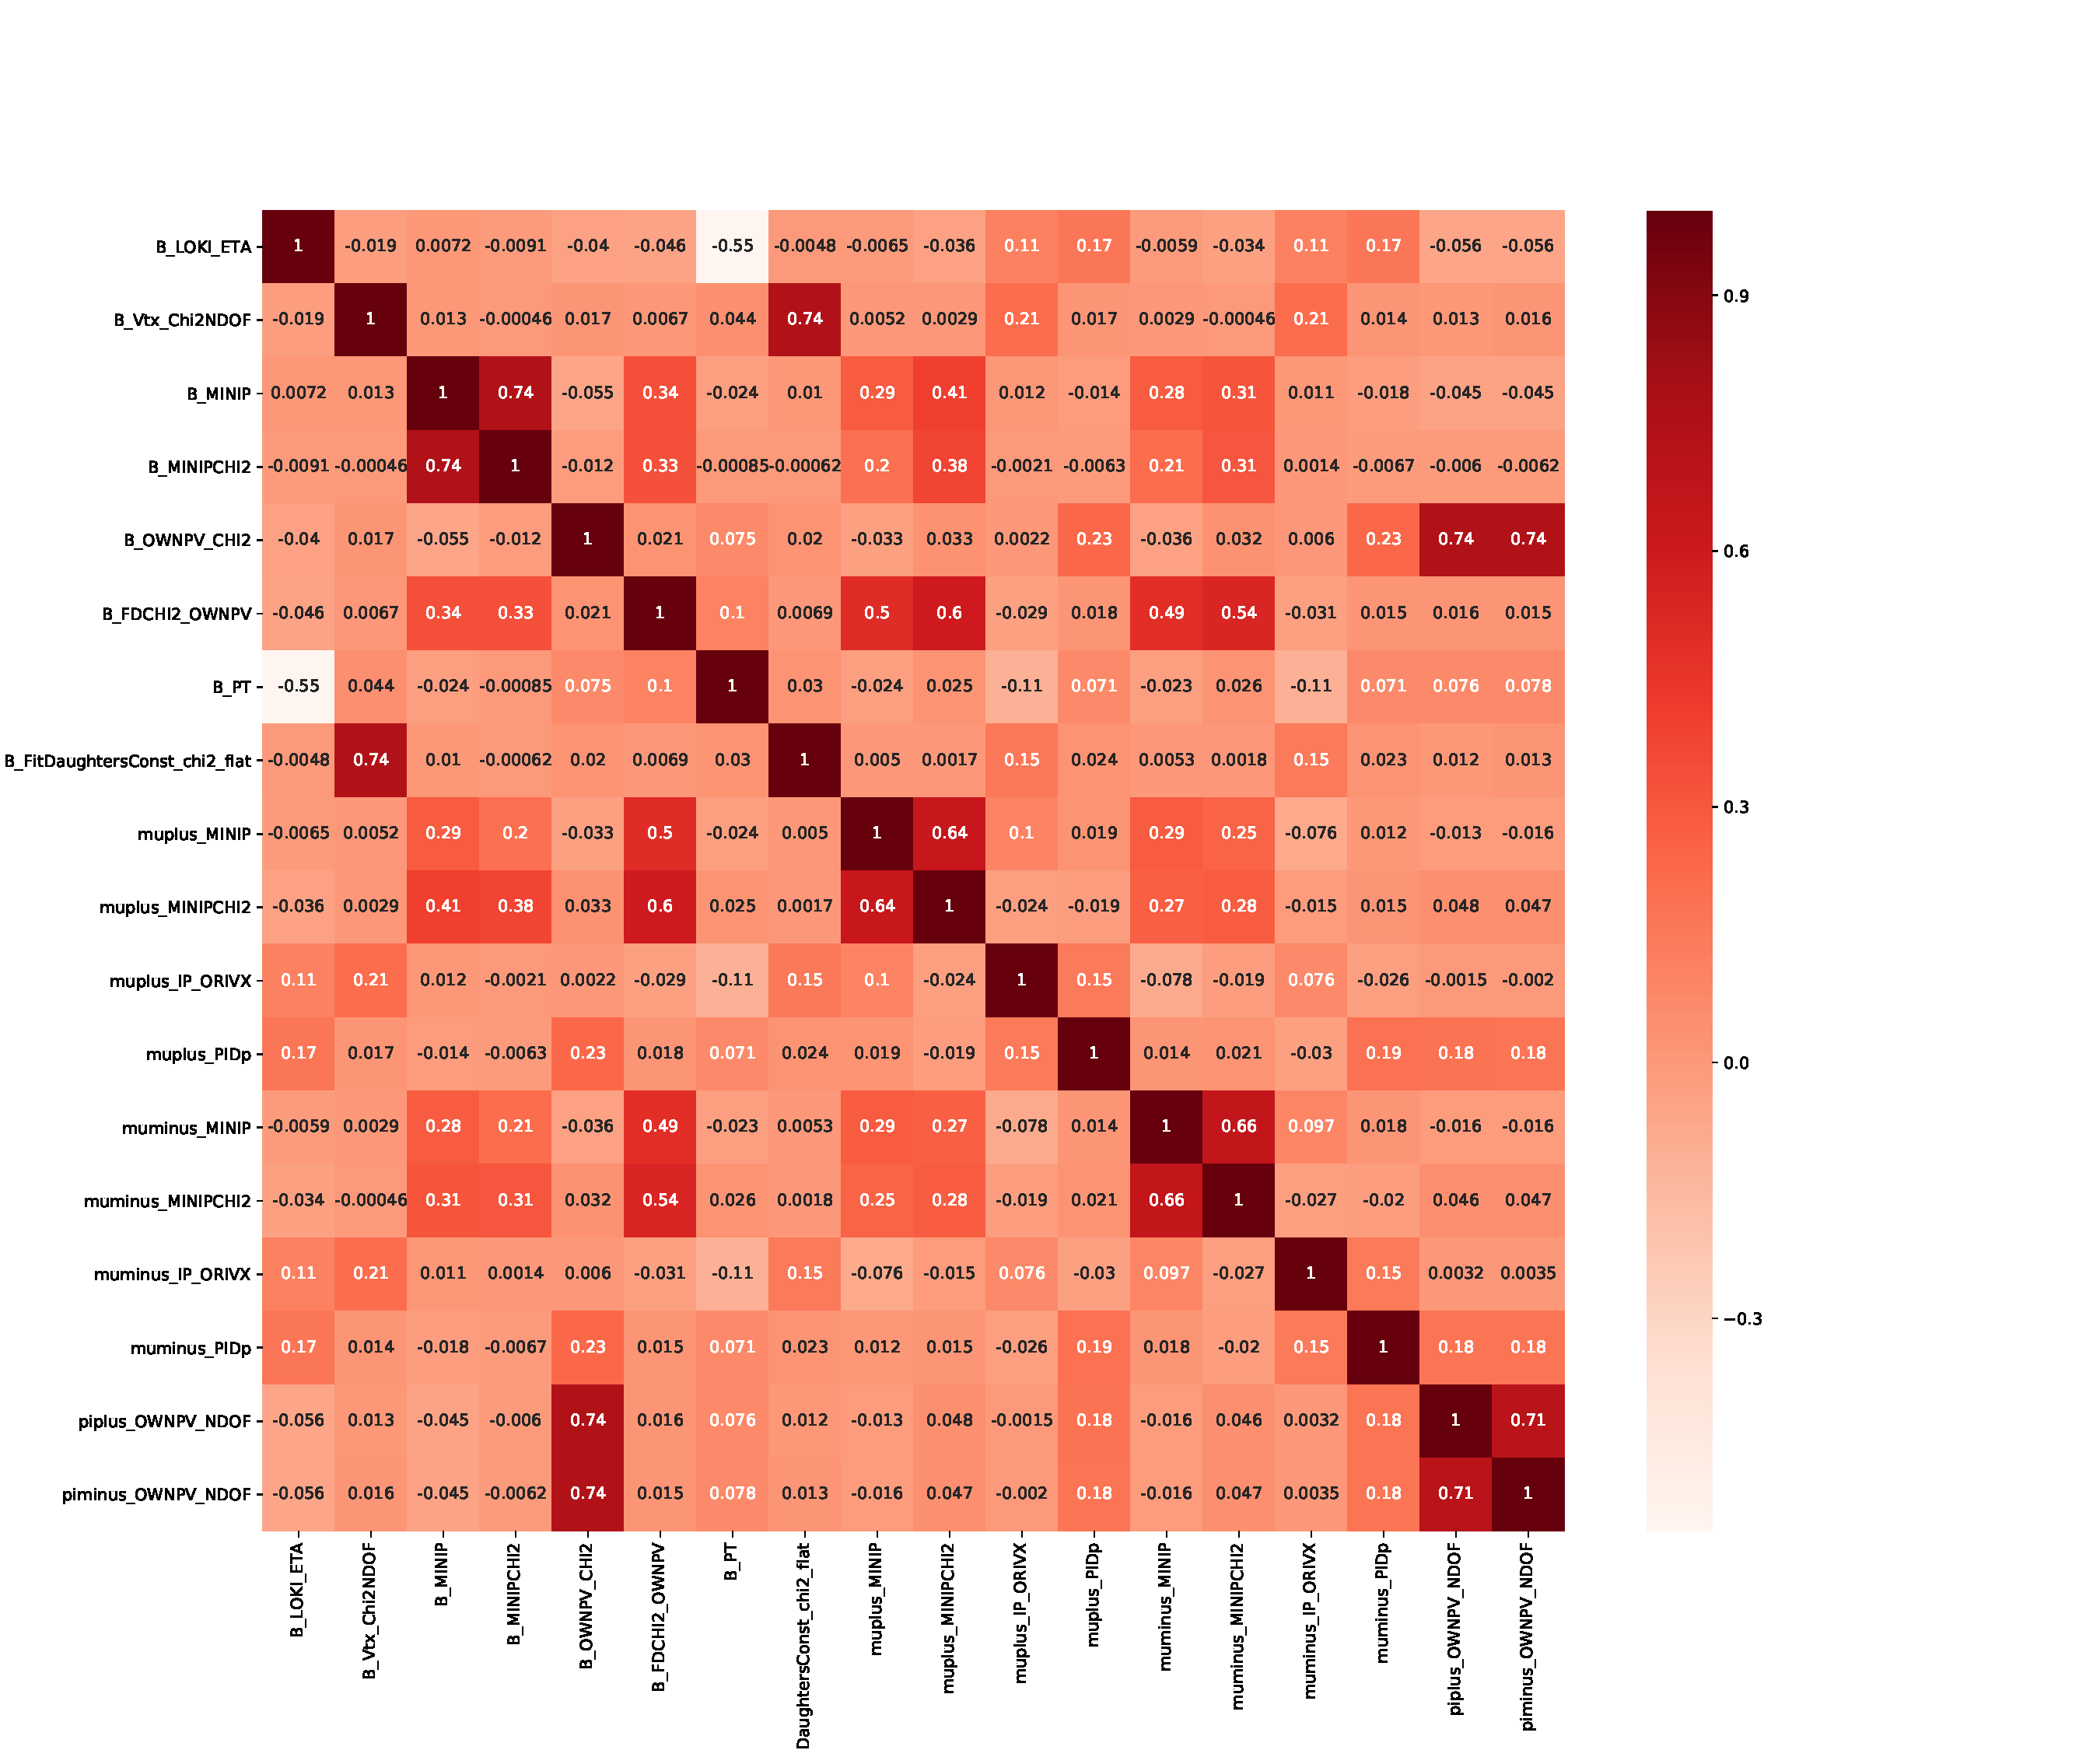
\includegraphics[width = .9\textwidth]{"content/plots/correlations.pdf"}
  \caption{Correlations between the 10 selected variables and the reconstructed $B^0$ mass.}
  \label{fig:correlations}
\end{figure}

\subsection{Training of MVA classifier}

\begin{figure}
  \centering
  \begin{subfigure}[b]{0.45\textwidth}
    \centering
    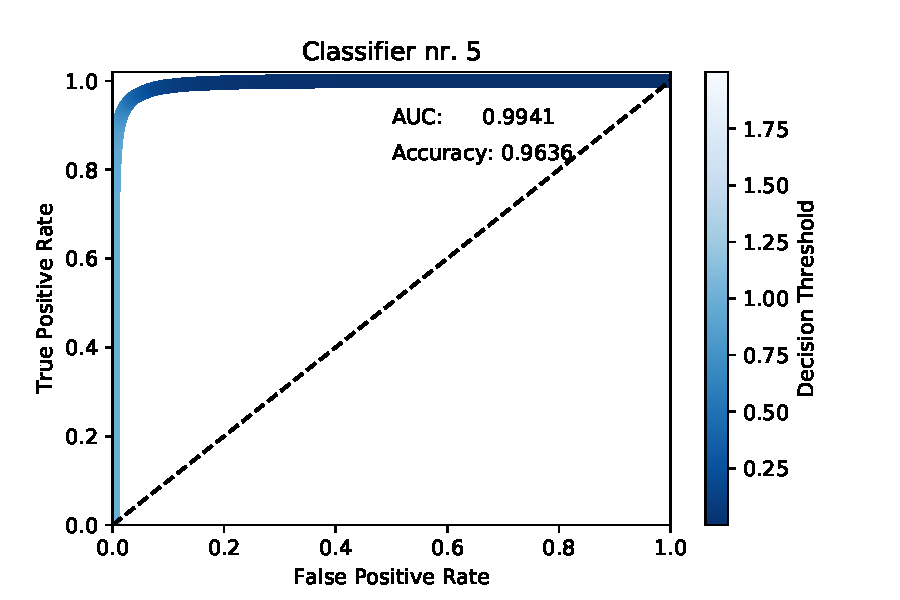
\includegraphics[width=\textwidth]{"content/plots/BDT_roc_auc.pdf"}
    %\caption{ROC curve.}
    \label{fig:roc_curve}
  \end{subfigure}
  \hfill
  \begin{subfigure}[b]{0.45\textwidth}
    \centering
    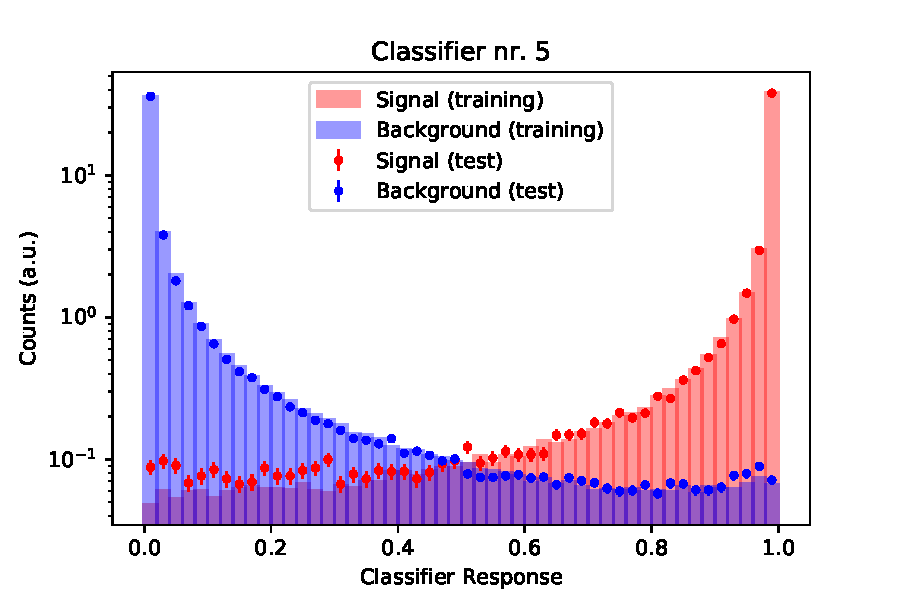
\includegraphics[width=\textwidth]{"content/plots/BDT_train_test.pdf"}
    %\caption{Performance on test vs. training dataset.}
    \label{fig:train_test}
  \end{subfigure}
  \caption{ROC curve (left) and performance on training and test dataset for one of the trained classifiers.}
  \label{fig:BDT}
\end{figure}

\subsection{Optimization of the classification threshold}

\begin{figure}
  \centering
  \begin{subfigure}[b]{0.45\textwidth}
    \centering
    \includegraphics[width=\textwidth]{"content/plots/pfom_full.pdf"}
    %\caption{ROC curve.}
  \end{subfigure}
  \hfill
  \begin{subfigure}[b]{0.45\textwidth}
    \centering
    \includegraphics[width=\textwidth]{"content/plots/pfom_zoom.pdf"}
  \end{subfigure}
  \caption{The Punzi figure of merit for the mean classifier response in different intervals of the threshold.}
  \label{fig:pFOM}
\end{figure}

\begin{figure}
  \centering
  \includegraphics[width = .8\textwidth]{"content/plots/mass_after_BDT.pdf"}
  \caption{Semi logarithmic invariant mass distribution of the $B^0$ candidates in data, after the cut on the classifier response is applied.}
  \label{fig:mass_after_BDT}
\end{figure}

\subsection{Evaluation of the signal yield}

\begin{figure}
  \centering
  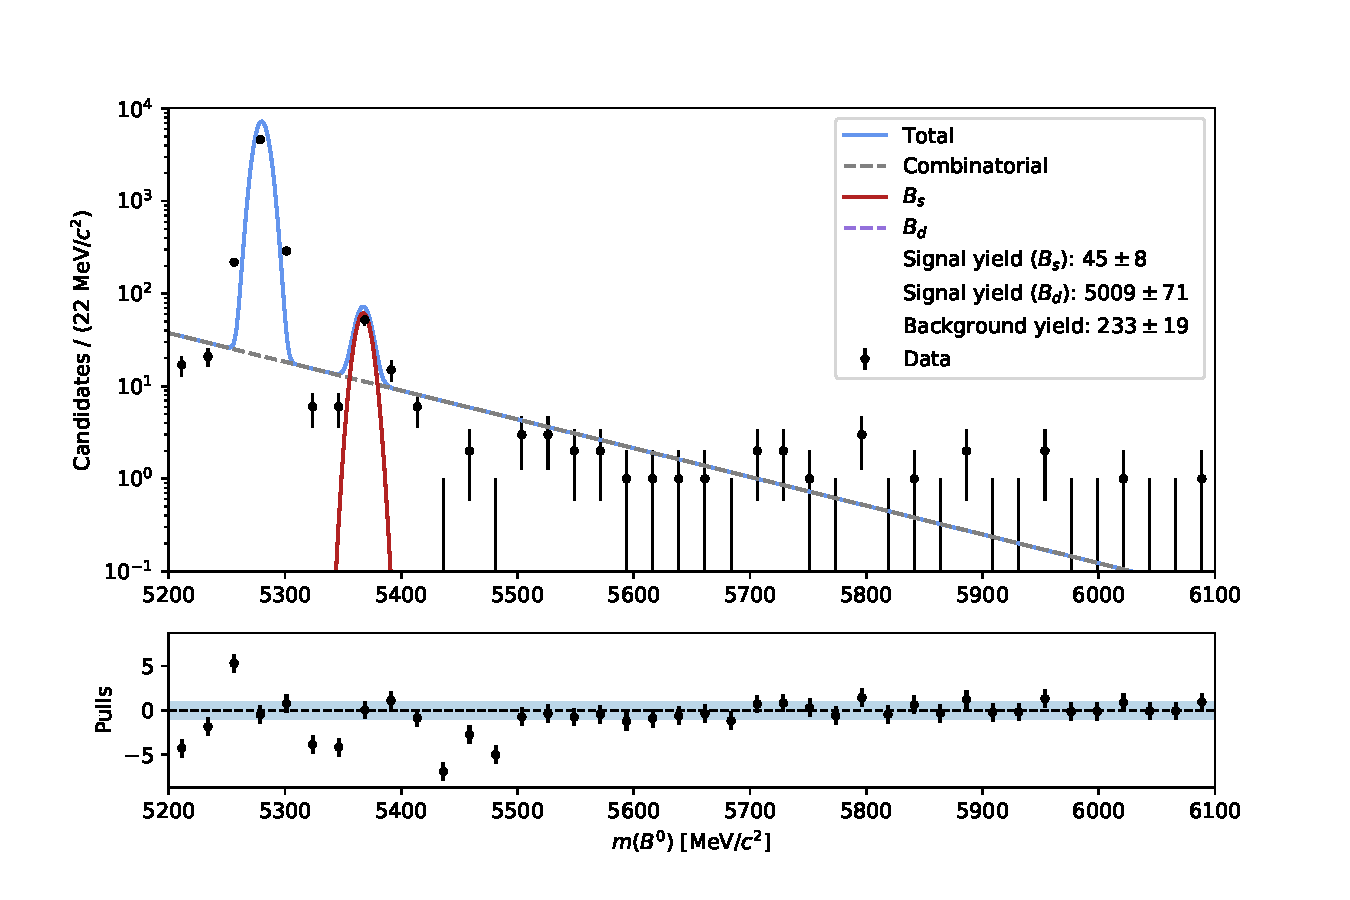
\includegraphics[width = .9\textwidth]{"content/plots/final_fit.pdf"}
  \caption{Fit to the invariant mass spectrum of the data in semi logarithmic depiction.}
  \label{fig:fit}
\end{figure}
